\documentclass{ximera}

\title{Activity: Calculus on Curves}
\author{Zack Reed}

\begin{document}
\begin{abstract}
In this activity we extend single-variable calculus ideas to vector functions.
\end{abstract}
\maketitle

\section*{Introduction: Vector Functions}

In single-variable settings, functions take numbers as inputs and produce numbers as outputs. 

\begin{center}
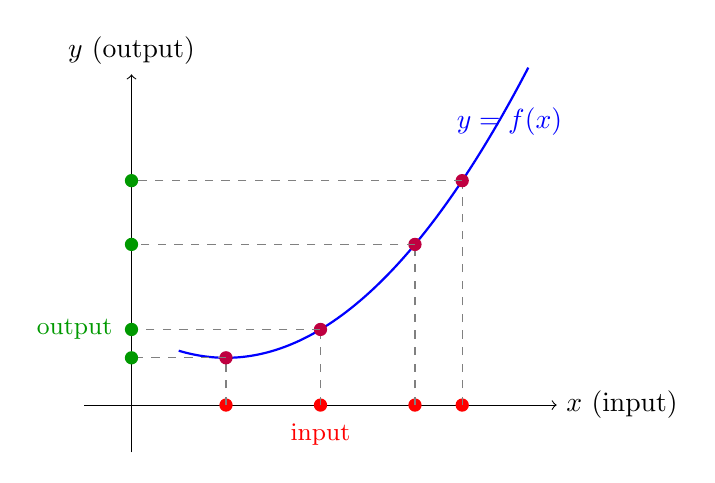
\begin{tikzpicture}[scale=1.2]
    % Draw axes
    \draw[->] (-0.5,0) -- (4.5,0) node[right] {$x$ (input)};
    \draw[->] (0,-0.5) -- (0,3.5) node[above] {$y$ (output)};
    
    % Draw the function curve y = 0.3(x-1)^2 + 0.5
    \draw[thick, blue, domain=0.5:4.2, samples=100] plot (\x, {0.3*(\x-1)^2 + 0.5});
    
    % Mark several input points
    \foreach \x/\y in {1/0.5, 2/0.8, 3/1.7, 3.5/2.375} {
        % Point on x-axis (input)
        \fill[red] (\x,0) circle (2pt);
        % Dashed line from x-axis to curve
        \draw[dashed, gray] (\x,0) -- (\x,\y);
        % Point on curve
        \fill[purple] (\x,\y) circle (2pt);
        % Dashed line from curve to y-axis
        \draw[dashed, gray] (\x,\y) -- (0,\y);
        % Point on y-axis (output)
        \fill[green!60!black] (0,\y) circle (2pt);
    }
    
    % Label the function
    \node[blue] at (4,3) {$y=f(x)$};
    
    % Add labels for one example
    \node[below, red, font=\small] at (2,-0.1) {input};
    \node[left, green!60!black, font=\small] at (-0.1,0.8) {output};
\end{tikzpicture}
\end{center}

In multivariable calculus, there are multiple variables as outputs, or multiple variables as inputs, or both!

Let's start with vector functions. These take in a single variable as input and produce a vector as output.

\begin{problem}
The geogebra applet breaks down a vector function that produces a simple helix, spiraling upward in 3D space.

\begin{expandable}{stuff}{GeoGebra Instructions}
    Rotate the 3D view by right-clicking and dragging on the right screen. 
    
    Drag the ``t='' slider on the top left to see the point move along the curve. You'll also see the values of each component function update as you change $t$.
\end{expandable}

\begin{center}
\geogebra{yxed8hcu}{730}{510}
\end{center}

There's no $t$ axis on the curve itself, but let's track what each component function is doing as $t$ changes.

Break down the curve by isolating each component with respect to time, but then also along each plane in 3D space.

\begin{enumerate}

\item The top left graph, showing how $z$ changes with $t$, is \wordChoice{\choice[correct]{linear}\choice{exponential}\choice{sine}\choice{cosine}}.

\item The middle left graph, showing how $y$ changes with $t$, is \wordChoice{\choice{linear}\choice{exponential}\choice[correct]{sine}\choice{cosine}}.

\item The bottom left graph, showing how $x$ changes with $t$, is \wordChoice{\choice{linear}\choice{exponential}\choice[correct]{cosine}\choice{sine}}.

\item If you right-click and drag the 3D view so that you're looking straight into the $x-z$ plane, the curve looks like a \wordChoice{\choice{line}\choice{circle}\choice{sine wave}\choice[correct]{cosine wave}}.

\item If you right-click and drag the 3D view so that you're looking straight into the $y-z$ plane, the curve looks like a \wordChoice{\choice{line}\choice{circle}\choice[correct]{sine wave}\choice{cosine wave}}.

\item If you right-click and drag the 3D view so that you're looking straight into the $x-y$ plane, the curve looks like a \wordChoice{\choice{line}\choice[correct]{circle}\choice{sine wave}\choice{cosine wave}}.

\end{enumerate}

\end{problem}

A key property of vector functions is that looking at the curve itself does not immediately indicate the component functions. Instead, the component functions determine how to vary along the curve as time passes.

\begin{definition}
A \textbf{vector function} is a function that produces a vector at each time in its domain.

The vector is defined by one scalar (single-variable) function for each component:
$$\vec{r}(t) = \langle x(t), y(t), z(t) \rangle = \langle f(t), g(t), h(t) \rangle, \quad \text{for } t \text{ in } [a,b]$$
\end{definition}

\begin{remark}
Vector functions are nice because we can work with each component function separately.
\end{remark}

The vector function for the helix in the applet is $\vec{r}(t) = [ \cos(t), \sin(t), t ]$.

\begin{problem}
Let's practice working with vector functions one component at a time. 

Answer the following questions about the vector functions. Note that these are functions of time, meaning that if we evaluate the vector function at a specific time $t$, we get a vector.

\begin{enumerate}
    \item For $\vec{r}(t) = [ t, t^2, t^3 ]$,
    \begin{itemize}
        \item $\vec{r}(1)$ is a \wordChoice{\choice{scalar}\choice[correct]{vector}\choice{graph}\choice{function}}.
        \item Which diagram correctly shows the vector $\vec{r}(1)$?
        \begin{multipleChoice}
            \choice[correct]{
                \begin{tikzpicture}[scale=0.6, thick, >=stealth]
                    \draw[->] (0,0,0) -- (1,1,1) node[above right] {$[1,1,1]$};
                    \draw[gray,dashed] (0,0,0) -- (2,0,0) node[right] {$x$};
                    \draw[gray,dashed] (0,0,0) -- (0,2,0) node[above] {$y$};
                    \draw[gray,dashed] (0,0,0) -- (0,0,2) node[below left] {$z$};
                    \fill (1,1,1) circle (2pt);
                \end{tikzpicture}
            }
            \choice{
                \begin{tikzpicture}[scale=0.6, thick, >=stealth]
                    \draw[->] (0,0,0) -- (1,0,1) node[above right] {$[1,0,1]$};
                    \draw[gray,dashed] (0,0,0) -- (2,0,0) node[right] {$x$};
                    \draw[gray,dashed] (0,0,0) -- (0,2,0) node[above] {$y$};
                    \draw[gray,dashed] (0,0,0) -- (0,0,2) node[below left] {$z$};
                    \fill (1,0,1) circle (2pt);
                \end{tikzpicture}
            }
            \choice{
                \begin{tikzpicture}[scale=0.6, thick, >=stealth]
                    \draw[->] (0,0,0) -- (1,-1,1) node[above right] {$[1,-1,1]$};
                    \draw[gray,dashed] (0,0,0) -- (2,0,0) node[right] {$x$};
                    \draw[gray,dashed] (0,0,0) -- (0,2,0) node[above] {$y$};
                    \draw[gray,dashed] (0,0,0) -- (0,0,2) node[below left] {$z$};
                    \fill (1,-1,1) circle (2pt);
                \end{tikzpicture}
            }
            \choice{
                \begin{tikzpicture}[scale=0.6, thick, >=stealth]
                    \draw[->] (0,0,0) -- (1,1,0) node[above right] {$[1,1,0]$};
                    \draw[gray,dashed] (0,0,0) -- (2,0,0) node[right] {$x$};
                    \draw[gray,dashed] (0,0,0) -- (0,2,0) node[above] {$y$};
                    \draw[gray,dashed] (0,0,0) -- (0,0,2) node[below left] {$z$};
                    \fill (1,1,0) circle (2pt);
                \end{tikzpicture}
            }
        \end{multipleChoice}
        \begin{feedback}
            Remember to evaluate each component of the vector function at $t=1$: $\vec{r}(1) = [1, 1^2, 1^3] = [1, 1, 1]$.
        \end{feedback}
        \item $\vec{r}(2) =  [ \answer{2}, \answer{4}, \answer{8}]$
        \item The $y$-component of $\vec{r}(3)$ is a \wordChoice{\choice[correct]{scalar}\choice{vector}\choice{graph}\choice{function}} with a value of $\answer{9}$.
    \end{itemize}
    
    \item If $\vec{s}(t) = [ \sin(t^2), e^t, \sqrt{t} ]$,
    \begin{itemize}
        \item $\vec{s}\left(0\right) = [ \answer{0}, \answer{1}, \answer{0} ]$
        \item The norm of $\vec{s}(1)$ is approximately $|\vec{s}(1)| \approx \answer[tolerance=1]{\sqrt{(\sin(1))^2 + e^2 + 1}}$
    \end{itemize}
\end{enumerate}

\begin{feedback}
As $t$ varies, the position vector $\vec{r}(t)$ traces out a path (curve) through 3D space. Think of it like a particle moving through space over time!
\end{feedback}
\end{problem}

You can also do vector operations on vector functions!

\begin{problem}
    Let's do some vector products on the vector functions $\vec{r}(t) = [ 2t, t^2, 3 ]$ and $\vec{s}(t) = [ \sin(t^2), e^t, \sqrt{t} ]$.
    
    First, let's evaluate at $t=2$:
    \begin{itemize}
        \item $\vec{r}(2) = [\answer{4}, \answer{4}, \answer{3}]$
        \item $\vec{s}(2) = [\sin(4), e^2, \sqrt{2}] \approx [-0.757, 7.389, 1.414]$
    \end{itemize}
    
    \begin{enumerate}
        \item Now compute the cross product $\vec{r}(2) \times \vec{s}(2)$ using the cross product formula:
        
        For $\vec{r}(2) = [4, 4, 3]$ and $\vec{s}(2) = [\sin(4), e^2, \sqrt{2}]$:
        
        $$\vec{r}(2) \times \vec{s}(2) = 
        \begin{bmatrix}
        r_2 s_3 - r_3 s_2 \\
        r_3 s_1 - r_1 s_3 \\
        r_1 s_2 - r_2 s_1
        \end{bmatrix}$$
        
        The $x$-component is: $r_2 s_3 - r_3 s_2 = \answer[tolerance=0.1]{4\sqrt{2} - 3e^2}$ (or approximately $\answer[tolerance=0.5]{-16.5}$)
        
        The $y$-component is: $r_3 s_1 - r_1 s_3 = \answer[tolerance=0.1]{3\sin(4) - 4\sqrt{2}}$ (or approximately $\answer[tolerance=0.5]{-8.4}$)
        
        The $z$-component is: $r_1 s_2 - r_2 s_1 = \answer[tolerance=0.1]{4e^2 - 4\sin(4)}$ (or approximately $\answer[tolerance=0.5]{32.6}$)
        
        \begin{feedback}
            Remember the cross product formula for $\vec{a} = [a_1, a_2, a_3]$ and $\vec{b} = [b_1, b_2, b_3]$:
            $$\vec{a} \times \vec{b} = 
            \begin{bmatrix}
            a_2 b_3 - a_3 b_2 \\
            a_3 b_1 - a_1 b_3 \\
            a_1 b_2 - a_2 b_1
            \end{bmatrix}$$
        \end{feedback}
        
        \item The cross product $\vec{r}(2)\times \vec{s}(2)$ produces a vector that is perpendicular to both $\vec{r}(2)$ and $\vec{s}(2)$. Which diagram correctly shows the cross product vector?
        \begin{multipleChoice}
            \choice{
                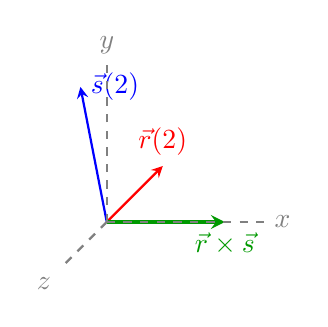
\begin{tikzpicture}[scale=0.5, thick, >=stealth]
                    % Input vectors
                    \draw[->, red] (0,0,0) -- (2,2,1.5) node[above] {$\vec{r}(2)$};
                    \draw[->, blue] (0,0,0) -- (-0.4,3.7,0.7) node[right] {$\vec{s}(2)$};
                    % Wrong result - parallel to xy-plane
                    \draw[->, green!60!black, very thick] (0,0,0) -- (3,0,0) node[below] {$\vec{r}\times\vec{s}$};
                    % Axes
                    \draw[gray,dashed] (0,0,0) -- (4,0,0) node[right] {$x$};
                    \draw[gray,dashed] (0,0,0) -- (0,4,0) node[above] {$y$};
                    \draw[gray,dashed] (0,0,0) -- (0,0,3) node[below left] {$z$};
                \end{tikzpicture}
            }
            \choice[correct]{
                \begin{tikzpicture}[scale=0.5, thick, >=stealth]
                    % Input vectors
                    \draw[->, red] (0,0,0) -- (2,2,1.5) node[above] {$\vec{r}(2)$};
                    \draw[->, blue] (0,0,0) -- (-0.4,3.7,0.7) node[right] {$\vec{s}(2)$};
                    % Correct result - perpendicular to both
                    \draw[->, green!60!black, very thick] (0,0,0) -- (-2.5,-2,8) node[right] {$\vec{r}\times\vec{s}$};
                    % Axes
                    \draw[gray,dashed] (0,0,0) -- (4,0,0) node[right] {$x$};
                    \draw[gray,dashed] (0,0,0) -- (0,4,0) node[above] {$y$};
                    \draw[gray,dashed] (0,0,0) -- (0,0,3) node[below left] {$z$};
                \end{tikzpicture}
            }
            \choice{
                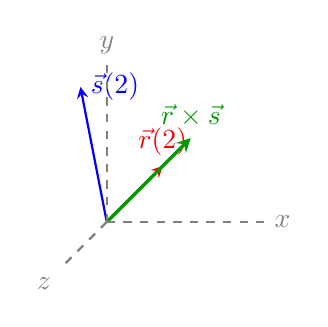
\begin{tikzpicture}[scale=0.5, thick, >=stealth]
                    % Input vectors
                    \draw[->, red] (0,0,0) -- (2,2,1.5) node[above] {$\vec{r}(2)$};
                    \draw[->, blue] (0,0,0) -- (-0.4,3.7,0.7) node[right] {$\vec{s}(2)$};
                    % Wrong result - along one of the input vectors
                    \draw[->, green!60!black, very thick] (0,0,0) -- (3,3,2.25) node[above] {$\vec{r}\times\vec{s}$};
                    % Axes
                    \draw[gray,dashed] (0,0,0) -- (4,0,0) node[right] {$x$};
                    \draw[gray,dashed] (0,0,0) -- (0,4,0) node[above] {$y$};
                    \draw[gray,dashed] (0,0,0) -- (0,0,3) node[below left] {$z$};
                \end{tikzpicture}
            }
            \choice{
                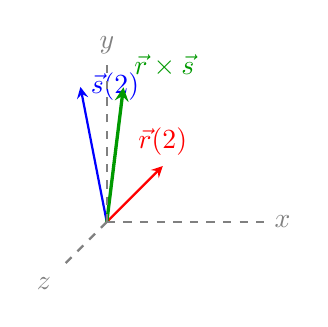
\begin{tikzpicture}[scale=0.5, thick, >=stealth]
                    % Input vectors
                    \draw[->, red] (0,0,0) -- (2,2,1.5) node[above] {$\vec{r}(2)$};
                    \draw[->, blue] (0,0,0) -- (-0.4,3.7,0.7) node[right] {$\vec{s}(2)$};
                    % Wrong result - in the plane of the two vectors
                    \draw[->, green!60!black, very thick] (0,0,0) -- (1,4,1.5) node[above right] {$\vec{r}\times\vec{s}$};
                    % Axes
                    \draw[gray,dashed] (0,0,0) -- (4,0,0) node[right] {$x$};
                    \draw[gray,dashed] (0,0,0) -- (0,4,0) node[above] {$y$};
                    \draw[gray,dashed] (0,0,0) -- (0,0,3) node[below left] {$z$};
                \end{tikzpicture}
            }
        \end{multipleChoice}
        \begin{feedback}
            The cross product $\vec{a} \times \vec{b}$ produces a vector perpendicular to both $\vec{a}$ and $\vec{b}$. The correct result has negative $x$ and $y$ components but a large positive $z$ component: approximately $[-16.5, -8.4, 32.6]$.
        \end{feedback}
        
        \item Now compute the dot product: $\vec{r}(1) \cdot \vec{s}(1) = \answer[tolerance=1]{2\sin(1) + e + 3}$
        
        \begin{feedback}
            For the dot product, evaluate each vector at $t=1$: $\vec{r}(1) = [2, 1, 3]$ and $\vec{s}(1) = [\sin(1), e, 1]$. Then compute: $2\sin(1) + 1 \cdot e + 3 \cdot 1 \approx 6.40$.
        \end{feedback}
    \end{enumerate}
    \begin{feedback}
    Remember to evaluate each vector function at the specified $t$ value before performing the vector operations! You treat the outputs of the functions as regular vectors.
    \end{feedback}
\end{problem}

\section*{Task One: Tangent Vectors and Velocity}

\subsection*{From Single-Variable to Vector Derivatives}

Because we can work with each component separately, differentiating vector functions is straightforward: differentiate each component!

\begin{problem}
Let's review the single-variable case first. In Calc I and II, we measured instantaneous rate of change by taking derivatives.

For a function $f(x)$, the derivative $f'(x)$ tells us:
\begin{selectAll}
    \choice[correct]{The instantaneous rate of change}
    \choice[correct]{The slope of the tangent line}
    \choice{The area under the curve}
    \choice[correct]{How fast the function is changing}
\end{selectAll}

\begin{feedback}
The derivative captures instantaneous rate of change. Now we'll extend this idea to vector functions!
\end{feedback}
\end{problem}

\begin{problem}
Before viewing the next applet, let's explore the 2D case.

\begin{expandable}{stuff}{GeoGebra Instructions}
    Alter the ``X='' slider to see the tangent line shift along the curve. Notice the approximating horizontal and vertical components represented by $dx$ and $df$.
\end{expandable}

\begin{center}
\geogebra{gyh4uhzy}{786}{584}
\end{center}

What does the tangent line represent?
\begin{multipleChoice}
    \choice{The curve itself}
    \choice[correct]{The direction and rate of change at a specific point}
    \choice{The average rate of change}
    \choice{The total change over an interval}
\end{multipleChoice}
\end{problem}

\subsection*{Computing Velocity Vectors}

\begin{definition}
For a vector function $\vec{r}(t) = \langle x(t), y(t), z(t) \rangle$, the \textbf{velocity vector} (or \textbf{tangent vector}) is:
$$\vec{v}(t) = \vec{r}'(t) = \left\langle \frac{dx}{dt}, \frac{dy}{dt}, \frac{dz}{dt} \right\rangle = \langle x'(t), y'(t), z'(t) \rangle$$

This vector is tangent to the curve and points in the direction of motion.
\end{definition}

\begin{problem}
Let's compute some velocity vectors. If $\vec{r}(t) = \langle t^2, 3t, 2t^3 \rangle$, find $\vec{v}(t)$.

$\vec{v}(t) = \langle \answer{2t}, \answer{3}, \answer{6t^2} \rangle$

At $t=1$: $\vec{v}(1) = \langle \answer{2}, \answer{3}, \answer{6} \rangle$

At $t=2$: $\vec{v}(2) = \langle \answer{4}, \answer{3}, \answer{24} \rangle$

\begin{feedback}
Notice how the velocity vector changes as $t$ changes! At $t=2$, the particle is moving much faster in the $z$-direction than at $t=1$.
\end{feedback}
\end{problem}

\begin{problem}
For the helix $\vec{r}(t) = \langle \cos(t), \sin(t), t \rangle$, compute the velocity vector.

$\vec{v}(t) = \langle \answer{-\sin(t)}, \answer{\cos(t)}, \answer{1} \rangle$

\begin{feedback}
The $z$-component of velocity is constantly 1, meaning the helix rises at a constant rate. The $x$ and $y$ components oscillate, creating the circular motion.
\end{feedback}
\end{problem}

\begin{problem}
Now visualize how the velocity vector moves along the curve in 3D.

\begin{expandable}{stuff}{GeoGebra Instructions}
    Alter the ``t='' slider to view the velocity vector at different points. Click and drag to rotate your view. Notice how the vector is always tangent to the curve.
\end{expandable}

\begin{center}
\geogebra{zr86834p}{730}{487}
\end{center}

After exploring the visualization, answer:
\begin{selectAll}
    \choice[correct]{The velocity vector is always tangent to the curve}
    \choice[correct]{The velocity vector's direction changes as the particle moves}
    \choice{The velocity vector is always the same length}
    \choice[correct]{The velocity vector points in the direction of motion}
\end{selectAll}
\end{problem}

\section*{Task Two: Integrating Vector Functions}

\subsection*{Reconstructing Position from Velocity}

In single-variable calculus, we learned that integration adds up little bits of products, such as rate-time products $r\cdot dt$ to accumulate a quantity, like distance. We did this using the Fundamental Theorem of Calculus, which leverages \emph{antiderivatives}.

The same is true for integrating vector functions, but you can choose to set up the adding up pieces in a few ways. The first, and easiest, is to add up pieces within each component, meaning we use the FTC on each component individually.

\begin{problem}
Let's review: In single-variable calculus, if a rocket has velocity $v(t)$ over time interval $[a,b]$, the total change in height is:

\begin{multipleChoice}
    \choice{$v(b) - v(a)$}
    \choice[correct]{$\int_a^b v(t) \, dt$}
    \choice{$v(b) \cdot (b-a)$}
    \choice{$\frac{dv}{dt}$}
\end{multipleChoice}

\begin{feedback}
We integrate velocity to find displacement! Small bits of distance $dD = v(t) \cdot dt$ add up to give total change: $\Delta D = \int_a^b v(t) \, dt$.
\end{feedback}
\end{problem}

\begin{problem}
Let's visualize this with a rocket example.

\begin{expandable}{stuff}{GeoGebra Instructions}
    Alter the ``t='' slider to view the rocket's height and velocity simultaneously. Notice how velocity determines the rate at which height accumulates.
\end{expandable}

\begin{center}
\geogebra{ysumvptx}{750}{467}
\end{center}

The rocket's velocity determines its motion, and total height accumulates over time. For instance, a height of $1090.2$ meters over $5.57$ seconds comes from: $1090.2 = \int_0^{5.57} v(t) \, dt$.

\begin{feedback}
Watch how the area under the velocity curve corresponds to the height gained. This is the fundamental theorem of calculus in action!
\end{feedback}
\end{problem}

\subsection*{Vector Integration: Component by Component}

\begin{definition}
For a vector velocity function $\vec{v}(t)=\langle x'(t), y'(t), z'(t)\rangle$, the change in position over $[a,b]$ is:
$$\vec{r}(b)-\vec{r}(a)= \int_a^b \vec{v}(t)\, dt=\left\langle \int_a^b x'(t)\, dt, \int_a^b y'(t)\, dt, \int_a^b z'(t)\, dt\right\rangle$$

We integrate each component separately!
\end{definition}

\begin{problem}
Key insight: When we integrate a vector function, what do we get?

\begin{multipleChoice}
    \choice{A scalar (number)}
    \choice[correct]{A vector representing the net change in position}
    \choice{The arc length}
    \choice{The speed}
\end{multipleChoice}

\begin{feedback}
Unlike scalar integration which gives a number, vector integration gives us a vector resulting from the accumulated displacements from the velocities across the time interval, showing the overall change in position!
\end{feedback}
\end{problem}

\begin{problem}
Let's practice! If $\vec{v}(t) = \langle 2, 3t, 4t^2 \rangle$, find the net position after starting at $\vec{r}(0) = \langle 0, 0, 0 \rangle$ and accumulating displacements from $t=0$ to $t=2$.

$\int_0^2 \vec{v}(t) \, dt = \left\langle \int_0^2 \answer{2} \, dt, \int_0^2 \answer{3t} \, dt, \int_0^2 \answer{4t^2} \, dt \right\rangle$

$= \langle \answer{4}, \answer{6}, \answer{32/3} \rangle$

\begin{feedback}
Remember: $\int_0^2 2 \, dt = 2t \big|_0^2 = 4$, $\int_0^2 3t \, dt = \frac{3t^2}{2} \big|_0^2 = 6$, and $\int_0^2 4t^2 \, dt = \frac{4t^3}{3} \big|_0^2 = \frac{32}{3}$.
\end{feedback}
\end{problem}

\begin{problem}
Now visualize this process in 3D.

\begin{expandable}{stuff}{GeoGebra Instructions}
    Alter the ``T='' slider to watch $\vec{r}$ build progressively by integrating each component. Observe how each coordinate changes independently.
\end{expandable}

\begin{center}
\geogebra{excy8qtq}{730}{510}
\end{center}

After exploring, select the true statements:
\begin{selectAll}
    \choice[correct]{Each component is integrated separately}
    \choice[correct]{The result is a displacement vector}
    \choice{The result tells us the arc length traveled}
    \choice[correct]{The process reconstructs position from velocity}
\end{selectAll}
\end{problem}

\section*{Task Three: Arc Length}

\subsection*{Distance vs. Displacement}

While integrating components gives us a function showing the resulting vectors from displacement up to a certain time, we often want to know the actual distance traveled along the curve—the arc length.

\begin{problem}
Think about the difference between displacement and distance:

If you walk 3 meters east, then 4 meters north, your displacement is:
\begin{multipleChoice}
    \choice{7 meters}
    \choice[correct]{5 meters (by Pythagorean theorem)}
    \choice{3 meters}
    \choice{4 meters}
\end{multipleChoice}

But the actual distance you walked is:
\begin{multipleChoice}
    \choice{5 meters}
    \choice[correct]{7 meters}
    \choice{3 meters}
    \choice{4 meters}
\end{multipleChoice}

\begin{feedback}
Displacement measures the straight-line change from start to finish. Distance measures the actual path length traveled. For curves, we use arc length to measure distance!
\end{feedback}
\end{problem}

\subsection*{Building the Arc Length Formula}

We've already learned about arc length in Calc II! Now we extend it to higher dimensions using the Pythagorean theorem.

\begin{problem}
Let's review the 2D case first. Explore the visualization below.

\begin{expandable}{stuff}{GeoGebra Instructions}
    Alter the ``x='' slider to see how small segments of the curve can be approximated by straight line segments. Notice the Pythagorean calculation.
\end{expandable}

\begin{center}
\geogebra{pd8zaw8v}{786}{584}
\end{center}

After exploring, what represents a small bit of arc length?
\begin{multipleChoice}
    \choice{$dx + dy$}
    \choice[correct]{$ds = \sqrt{(dx)^2 + (dy)^2}$}
    \choice{$dx \cdot dy$}
    \choice{$\frac{dy}{dx}$}
\end{multipleChoice}

\begin{feedback}
The Pythagorean theorem gives us the length of the small segment: $ds = \sqrt{(dx)^2 + (dy)^2}$!
\end{feedback}
\end{problem}

\begin{definition}
For a 2D curve with coordinate functions $x(t)$ and $y(t)$, a small arc length element is:
$$ds=\sqrt{\left(\frac{dx}{dt}\right)^2+\left(\frac{dy}{dt}\right)^2} \, dt=\sqrt{x'(t)^2+y'(t)^2} \, dt = |\vec{v}(t)| \, dt$$

The total arc length from $t=a$ to $t=b$ is:
$$L = \int_a^b ds = \int_a^b |\vec{v}(t)| \, dt = \int_a^b \sqrt{x'(t)^2+y'(t)^2} \, dt$$
\end{definition}

\begin{problem}
Key insight: What's the difference between $\int_a^b \vec{v}(t) \, dt$ and $\int_a^b |\vec{v}(t)| \, dt$?

$\int_a^b \vec{v}(t) \, dt$ gives:
\begin{multipleChoice}
    \choice{Arc length}
    \choice[correct]{Displacement (a vector)}
    \choice{Speed}
    \choice{Distance}
\end{multipleChoice}

$\int_a^b |\vec{v}(t)| \, dt$ gives:
\begin{multipleChoice}
    \choice{Displacement (a vector)}
    \choice[correct]{Arc length (distance traveled)}
    \choice{Velocity}
    \choice{Acceleration}
\end{multipleChoice}

\begin{feedback}
Without the magnitude bars, we integrate the vector to get displacement. With the magnitude bars, we integrate speed to get total distance (arc length)!
\end{feedback}
\end{problem}

\subsection*{Arc Length in 3D}

The same principle extends beautifully to 3D—we just add the $z$-component!

\begin{definition}
For a 3D curve $\vec{r}(t) = \langle x(t), y(t), z(t) \rangle$:
$$L = \int_a^b |\vec{v}(t)| \, dt = \int_a^b \sqrt{x'(t)^2+y'(t)^2+z'(t)^2} \, dt$$
\end{definition}

\begin{problem}
Let's compute an arc length! For $\vec{r}(t) = \langle 3t, 4t, 0 \rangle$ from $t=0$ to $t=2$:

First, find $\vec{v}(t) = \langle \answer{3}, \answer{4}, \answer{0} \rangle$

The speed is $|\vec{v}(t)| = \sqrt{9 + 16 + 0} = \answer{5}$

Since speed is constant, the arc length is simply:
$L = \int_0^2 5 \, dt = \answer{10}$

\begin{feedback}
When speed is constant, arc length is just speed times time! This curve is actually a straight line in the $xy$-plane moving at constant speed.
\end{feedback}
\end{problem}

\begin{problem}
Now for the helix $\vec{r}(t) = \langle \cos(t), \sin(t), t \rangle$ from $t=0$ to $t=2\pi$:

$\vec{v}(t) = \langle \answer{-\sin(t)}, \answer{\cos(t)}, \answer{1} \rangle$

$|\vec{v}(t)| = \sqrt{\sin^2(t) + \cos^2(t) + 1} = \answer{\sqrt{2}}$

The arc length for one complete turn is:
$L = \int_0^{2\pi} \sqrt{2} \, dt = \answer{2\pi\sqrt{2}}$ (or $\answer[tolerance=0.1]{8.886}$)

\begin{feedback}
The helix also has constant speed! Even though it's curving and rising, the total speed $\sqrt{2}$ remains constant.
\end{feedback}
\end{problem}

\begin{problem}
Visualize the 3D arc length calculation.

\begin{expandable}{stuff}{GeoGebra Instructions}
    Alter the ``t='' slider to see the arc length approximation at various points. Click, drag, and scroll to rotate and zoom. Select ``Reset Zoom'' or ``Zoom to Arc Length'' buttons for different views. Check ``Show x-y hypotenuse'' for more detail.
\end{expandable}

\begin{center}
\geogebra{nrnm8k7p}{780}{438}
\end{center}

After exploring, verify your understanding:
\begin{selectAll}
    \choice[correct]{Small arc length elements use the Pythagorean theorem in 3D}
    \choice[correct]{We integrate speed over time to get arc length}
    \choice{Arc length is always equal to displacement magnitude}
    \choice[correct]{Arc length measures actual distance traveled along the curve}
\end{selectAll}
\end{problem}

\section*{Summary: Two Types of Vector Integration}

We now have powerful tools for analyzing curves!

\begin{problem}
Let's review the two main ways we integrate vector functions:

\textbf{Type 1: Displacement (Vector Result)}
$$\vec{r}(b)-\vec{r}(a)= \int_a^b \vec{v}(t)\, dt=\left\langle \int_a^b x'(t)\, dt, \int_a^b y'(t)\, dt, \int_a^b z'(t)\, dt\right\rangle$$

This gives us:
\begin{multipleChoice}
    \choice{The distance traveled}
    \choice[correct]{The net change in position (displacement vector)}
    \choice{The speed}
    \choice{The arc length}
\end{multipleChoice}

\textbf{Type 2: Arc Length (Scalar Result)}
$$L = \int_a^b |\vec{v}(t)|\, dt=\int_a^b\sqrt{x'(t)^2+y'(t)^2+z'(t)^2}\, dt$$

This gives us:
\begin{multipleChoice}
    \choice{The displacement vector}
    \choice[correct]{The total distance traveled along the curve}
    \choice{The velocity}
    \choice{The final position}
\end{multipleChoice}

\begin{feedback}
These are fundamentally different! One integrates velocity (vector) to get displacement (vector). The other integrates speed (scalar) to get distance (scalar).
\end{feedback}
\end{problem}

\begin{problem}
Let's solidify understanding with a comprehensive example. Consider $\vec{r}(t) = \langle t, t^2, 2t \rangle$ from $t=0$ to $t=1$.

\textbf{Part A: Find the displacement}

$\int_0^1 \vec{v}(t) \, dt = \int_0^1 \langle \answer{1}, \answer{2t}, \answer{2} \rangle \, dt$

$= \langle \answer{1}, \answer{1}, \answer{2} \rangle$

\textbf{Part B: Find the arc length}

$|\vec{v}(t)| = \sqrt{1 + 4t^2 + 4} = \sqrt{\answer{5 + 4t^2}}$

The arc length requires numerical integration (this integral doesn't have a simple closed form):
$L = \int_0^1 \sqrt{5 + 4t^2} \, dt \approx \answer[tolerance=0.1]{2.46}$

\textbf{Part C: Compare}

The magnitude of the displacement is $|\langle 1, 1, 2 \rangle| = \sqrt{1+1+4} = \answer{\sqrt{6}} \approx 2.45$

Notice that the arc length ($\approx 2.46$) is slightly larger than the displacement magnitude ($\approx 2.45$). This makes sense because:
\begin{multipleChoice}
    \choice{Arc length should always be smaller}
    \choice[correct]{The curve isn't perfectly straight, so the path is slightly longer}
    \choice{We made a calculation error}
    \choice{They should be exactly equal}
\end{multipleChoice}

\begin{feedback}
The displacement gives the straight-line distance from start to finish. The arc length gives the actual distance traveled along the (slightly curved) path. The arc length is always greater than or equal to the displacement magnitude!
\end{feedback}
\end{problem}

\begin{problem}
Final check: Select all TRUE statements about vector calculus on curves.

\begin{selectAll}
    \choice[correct]{Velocity is the derivative of position}
    \choice[correct]{Velocity vectors are tangent to the curve}
    \choice[correct]{Integrating velocity gives displacement}
    \choice[correct]{Integrating speed gives arc length}
    \choice{Displacement and arc length are always equal}
    \choice[correct]{Arc length uses the Pythagorean theorem}
    \choice[correct]{We can work with vector functions component by component}
    \choice{The magnitude of displacement can exceed arc length}
\end{selectAll}

\begin{feedback}
Excellent! You've mastered the fundamentals of calculus on curves. These concepts—tangent vectors, integration, and arc length—are essential for understanding motion in space and will be the foundation for more advanced topics like curvature and TNB frames.
\end{feedback}
\end{problem}

\end{document}